% Career history supplied directly by Morgan Hough, September 5, 2026.
\section{My background}
\NTXDivider{About Me}
\begin{frame}{From Simple Systems Neurobiology\newline to HD-EEG \& Neuroimaging}
  \begin{columns}[c,onlytextwidth]
    \column{.61\textwidth}
      \fontsize{9.5}{11}\selectfont
      \textbf{A dual academic background}\par
      Biochemistry and molecular biology, alongside experimental psychology.\par\smallskip
      \textbf{Crustacean Behavioral Neurobiology Research Group}\par
      Started a student lab; built our own equipment to study operant conditioning in green crabs.\par\smallskip
      \textbf{After college: Karl Pribram}\par
      Worked on a novel high-density EEG system.\par\smallskip
      \textbf{Electrical Geodesics, Inc.}\par
      Worked under Don Tucker; later became software engineering manager.\par
    \column{.35\textwidth}
      \centering
      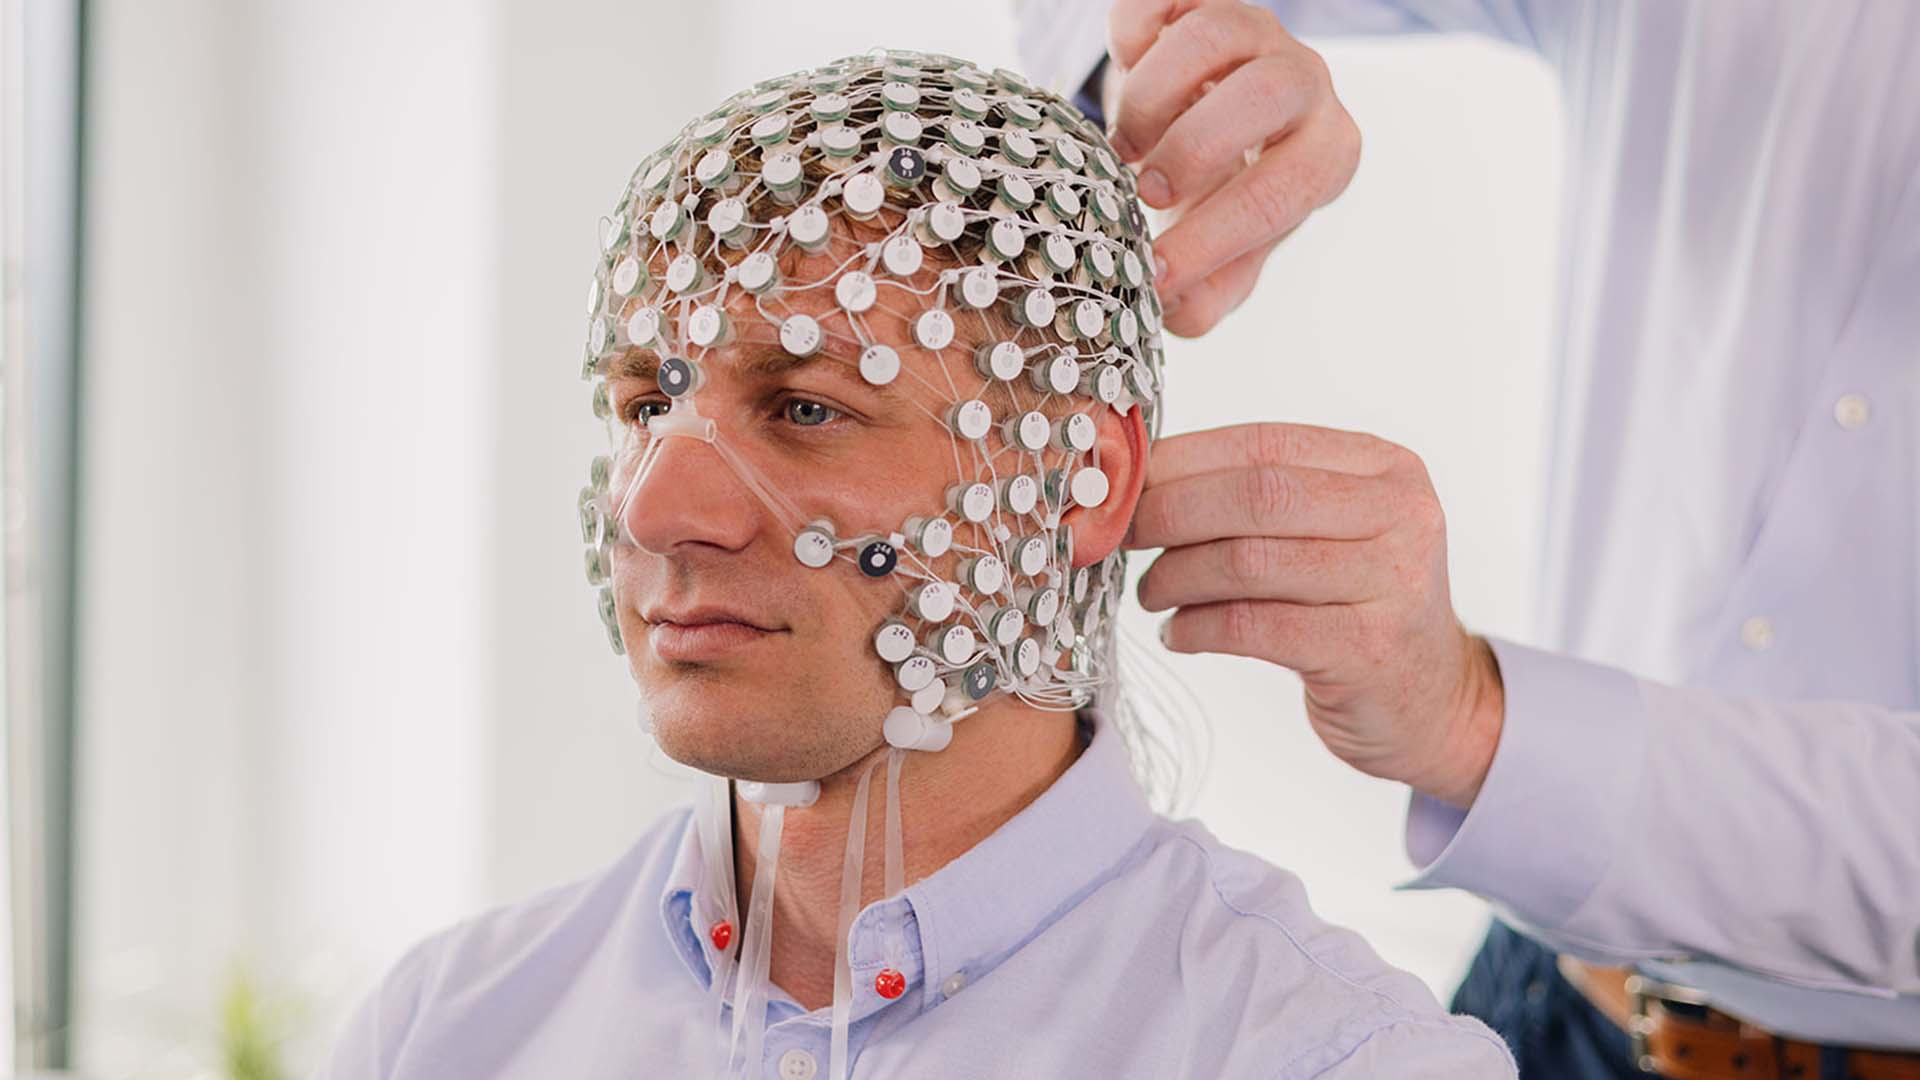
\includegraphics[width=\linewidth,height=20mm,keepaspectratio]{assets/history/egi-hd-eeg-sensor-net.jpg}
      \par{\tiny HD-EEG Geodesic Sensor Net\par}\smallskip
      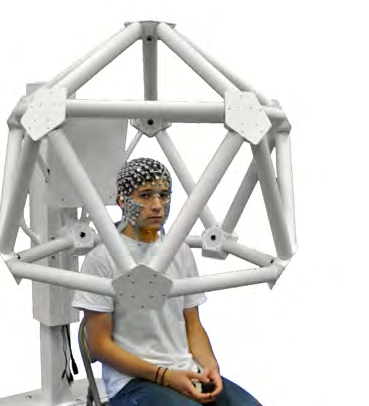
\includegraphics[width=\linewidth,height=22mm,keepaspectratio]{assets/history/egi-geodesic-camera-dome.png}
      \par{\tiny Geodesic Photogrammetry System\par}
  \end{columns}
  \smallskip{\tiny\color{NTXMuted}Equipment illustrations: \href{https://www.magstim.com/ges-500/}{Magstim EGI}; \href{https://www.egi.com/research-division/electrical-source-imaging/photogrammetry-sensor-digitization}{EGI sensor-digitization brochure}\par}
  \note{The right-hand images are official equipment illustrations, not Morgan or archival photos from his employment. The sensor-net photo comes from Magstim's GES 500 page; the camera dome was extracted from EGI's 2016 Sensor Digitization brochure. The Geodesic Photogrammetry System photographs electrode locations; it is distinct from the EEG sensor net. No claim is made that these particular product generations were the systems Morgan developed.}
  \note{[00:30--01:30] My academic background was dual: biochemistry and molecular biology, and experimental psychology. As a student I started the Crustacean Behavioral Neurobiology Research Group. We built our own equipment for studying operant conditioning in green crabs. This is an early example of the hands-on, collaborative approach that connects to the community-building story. After college I began working for Karl Pribram on a novel high-density EEG system. I was then hired by Electrical Geodesics, Inc., where I worked under Don Tucker and later became software engineering manager. The sequence and biographical details are supplied directly by Morgan; no degree titles, institutions, dates, or experimental results have been inferred.}
\end{frame}

\begin{frame}{UCSF and Oxford: neuroimaging methods}
  \begin{columns}[c,onlytextwidth]
    \column{.52\textwidth}
      \small
      \textbf{Dynamic Neuroimaging Lab, UCSF}\par
      Lab manager with Greg Simpson.\newline HD-EEG, MEG, and fMRI.\par\medskip
      \textbf{FMRIB, University of Oxford}\par
      Methods with Steve Smith and Mark Jenkinson in the Analysis Group.\par\medskip
      \textbf{Academic focus}\par
      Psychiatric applications of neuroimaging.\par\medskip
      \textbf{Physics-based head models}\par
      EEG, EIT, TES, TMS, and TFUS.\par
    \column{.44\textwidth}
      \centering
      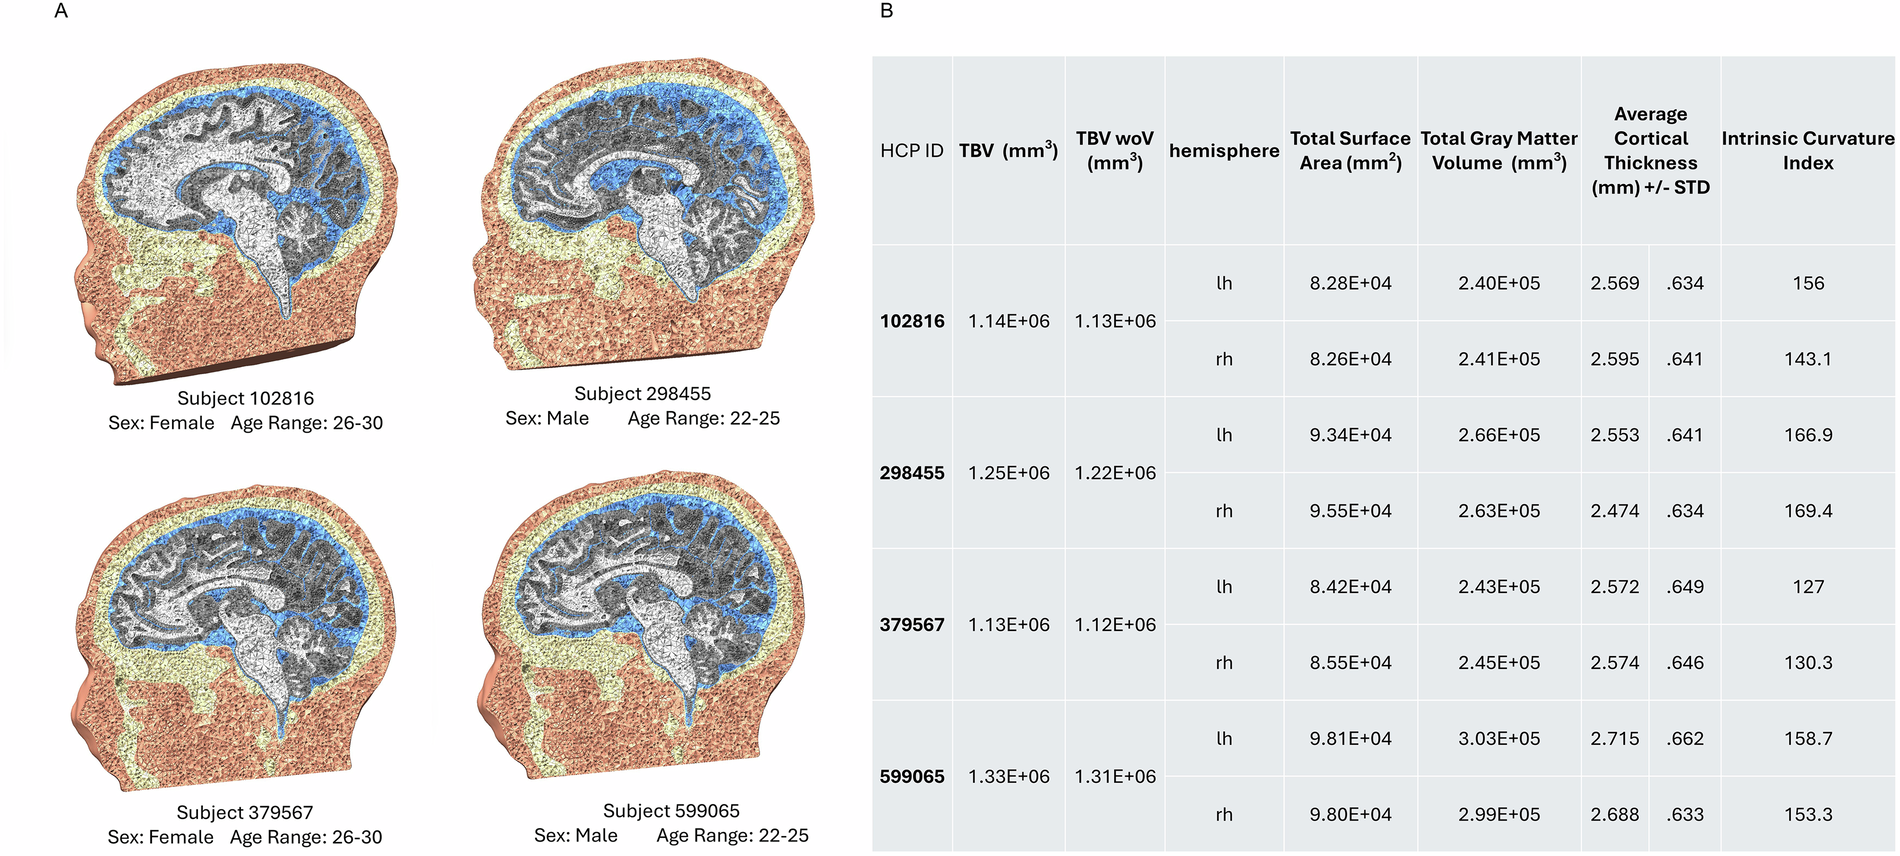
\includegraphics[trim=0bp 0bp 1040bp 0bp,clip,width=\linewidth,height=46mm,keepaspectratio]{assets/history/fem-berger-2025-fig2.png}
      \par\smallskip{\scriptsize MRI-derived finite-element head models\newline Skin, skull, CSF, eyes, gray and white matter\par}
  \end{columns}
  \smallskip{\tiny\color{NTXMuted}Image: \href{https://doi.org/10.1038/s41597-025-04886-0}{Berger et al., Scientific Data 12, 516 (2025), Fig.\ 2A}; cropped; \href{https://creativecommons.org/licenses/by/4.0/}{CC BY 4.0}\par}
  \note{Illustrative published finite-element head models, not Morgan's own results or Fijee output. Taylor A. Berger, Miles Wischnewski, Alexander Opitz, and Ivan Alekseichuk (2025), Human head models and populational framework for simulating brain stimulations, Scientific Data 12, 516, doi:10.1038/s41597-025-04886-0. Figure 2A shows four example subjects with six tissue types; subjects are not shown to scale. The slide crops out panel B's morphometric table without altering the models. Reused under CC BY 4.0.}
  \note{[01:30--02:30] At UCSF I was lab manager for the Dynamic Neuroimaging Lab under Greg Simpson, working with HD-EEG, MEG, and fMRI. At FMRIB, University of Oxford, I worked on methods development with Steve Smith and Mark Jenkinson in the Analysis Group. My academic work is primarily focused on psychiatric applications of neuroimaging. My technical expertise includes physics-based head models for EEG, EIT, TES, TMS, and TFUS. These descriptions are supplied directly by Morgan; they describe research focus and expertise, not claims of clinical efficacy or additional qualifications.}
\end{frame}

\begin{frame}{San Francisco: SKERI and Neuroscape}
  \begin{columns}[c,onlytextwidth]
    \column{.45\textwidth}
      \textbf{Smith Kettlewell Eye Research Institute}\par
      With Alex Wade\par\bigskip
      \textbf{Neuroscape at UCSF}\par
      With Adam Gazzaley
    \column{.51\textwidth}
      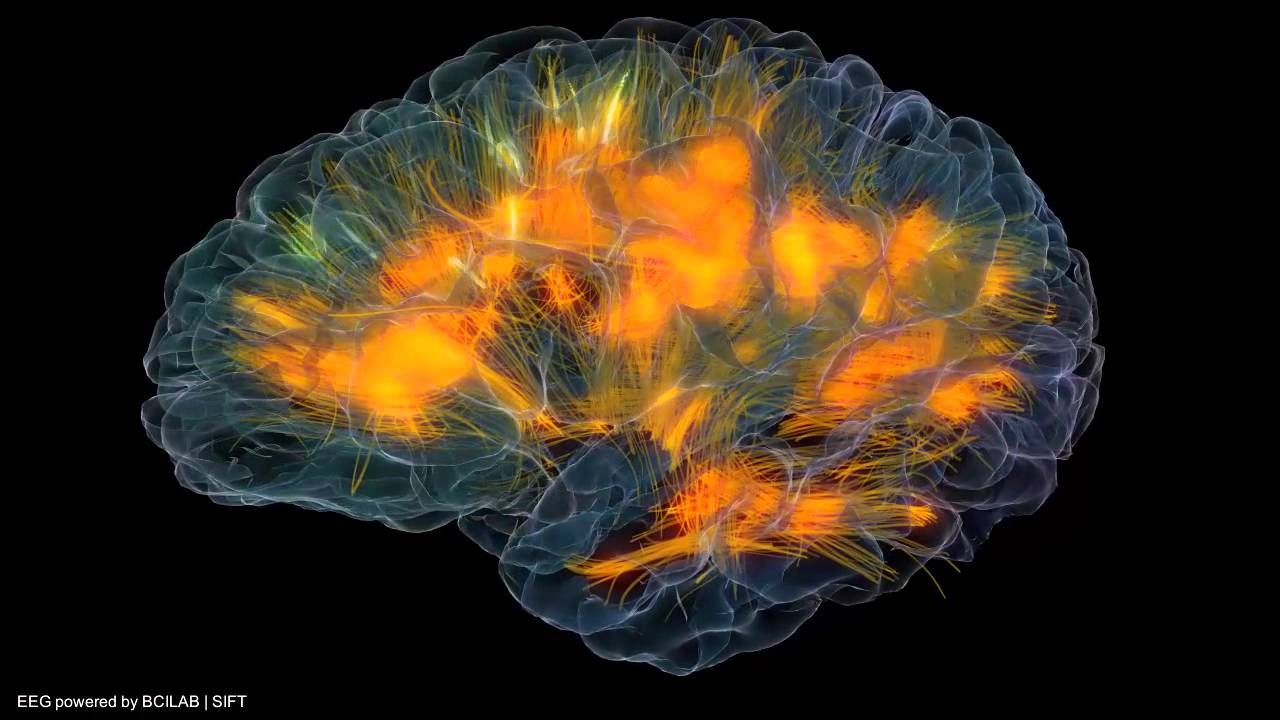
\includegraphics[width=\linewidth,height=43mm,keepaspectratio]{assets/history/neuroscape-glassbrain-video.jpg}
      \par\smallskip{\scriptsize Glass Brain --- MRI, diffusion imaging, and HD-EEG\newline Image: Neuroscape, UCSF\par}
  \end{columns}
  \smallskip{\tiny\color{NTXMuted}\href{https://neuroscape.ucsf.edu/technology/interventions-and-diagnostics/}{Neuroscape: Glass Brain}; \href{https://www.youtube.com/watch?v=dAIQeTeMJ-I}{official flythrough video}\par}
  \note{[02:30--03:00] After Oxford I returned to San Francisco: Smith Kettlewell Eye Research Institute with Alex Wade, then Neuroscape at UCSF with Adam Gazzaley. Glass Brain illustrates the Neuroscape setting: MRI and diffusion imaging provide anatomical context for HD-EEG activity visualization. This is the thumbnail of the official flythrough linked by Neuroscape, not a direct photograph of neural activity. Image credit: Neuroscape, UCSF. Their terms allow attributed non-commercial use but not commercial distribution or use as a presentation's primary feature. This supporting biography image is not the presentation's cover or central theme.}
\end{frame}

\begin{frame}{Back in San Francisco}
  \begin{columns}[c,onlytextwidth]
    \column{.55\textwidth}
      \small
      \textbf{Biopunk Lab}\par
      Founding Member --- synthetic neurobiology\par\smallskip
      \textbf{Neurotech@Frontier Tower}\par
      Lead\par\smallskip
      \textbf{Other Minds Lab}\par
      Co-founder\par\smallskip
      \textbf{Orthogonal Research \& DevoWorm Group}\par
      Lab Member\par\smallskip
      \textbf{NeuroTechX}\par
      Executive Director
    \column{.41\textwidth}
      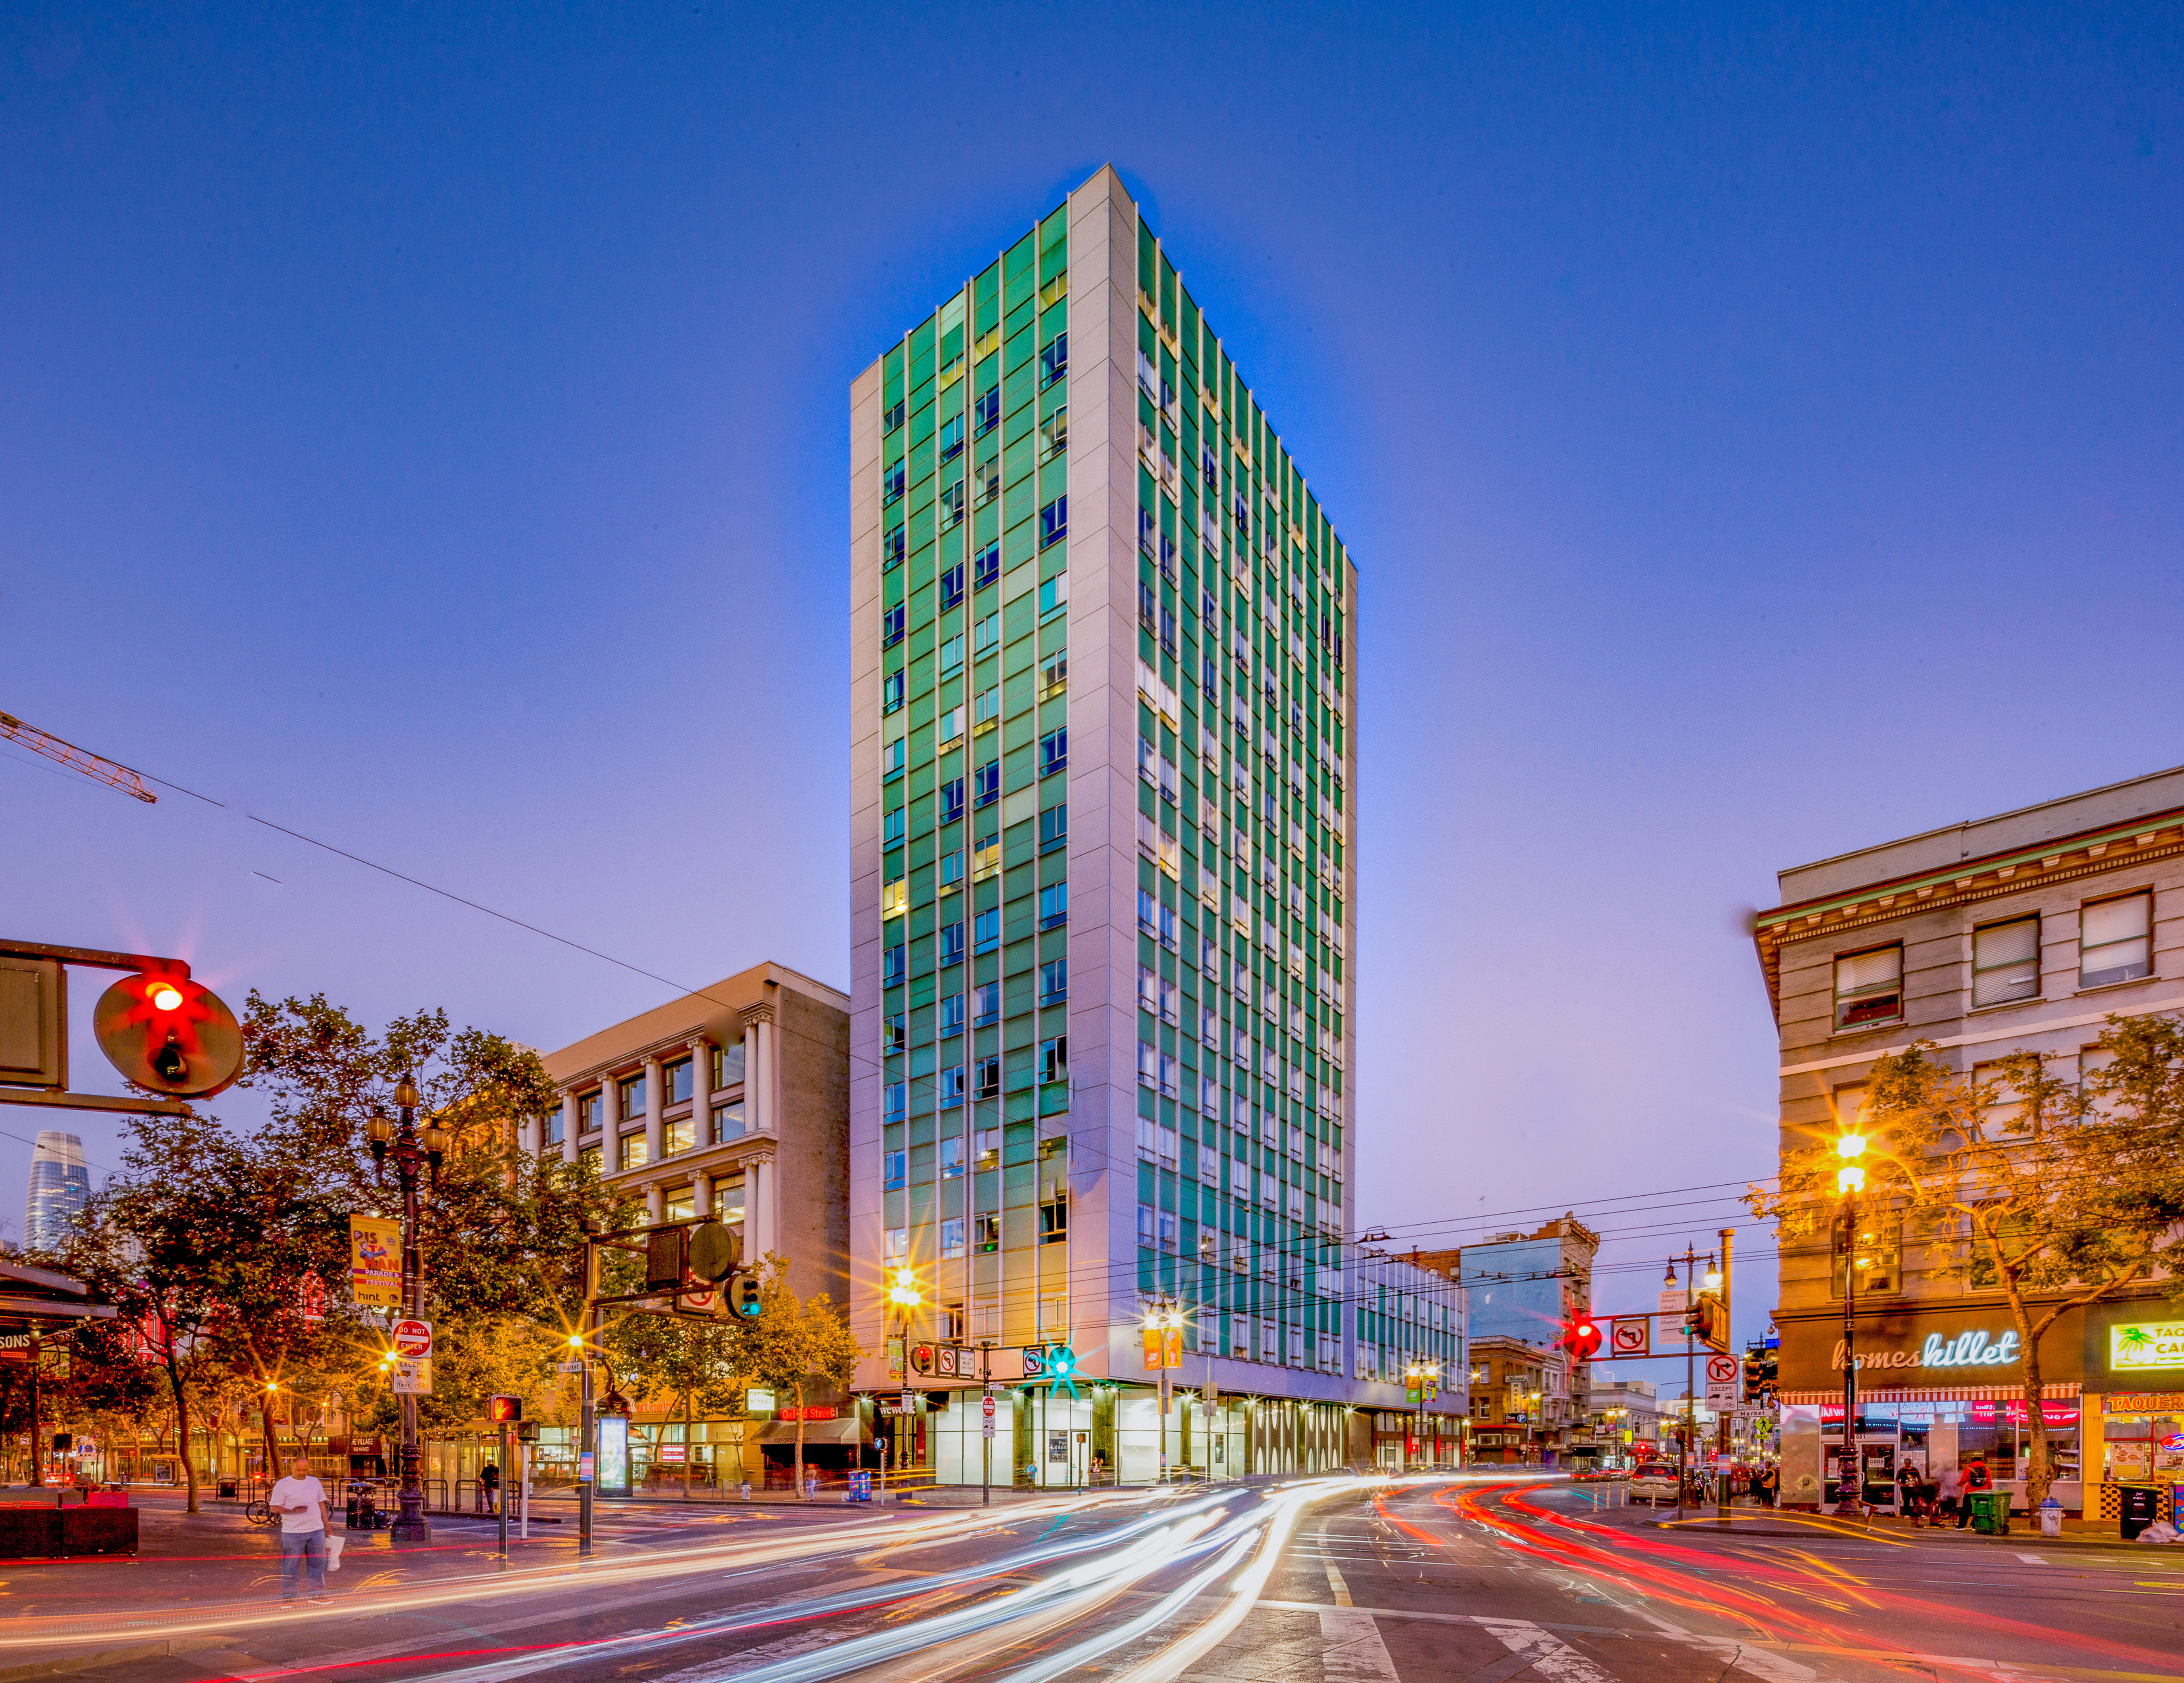
\includegraphics[width=\linewidth,height=52mm,keepaspectratio]{assets/history/frontier-tower-exterior.jpg}
      \par\smallskip
      {\tiny Frontier Tower, 995 Market Street\par
      Earlier exterior photo: \href{https://www.995market.com/}{Colliers / 995 Market listing}}
  \end{columns}
  \note{[03:00--03:30] I am a founding member of Biopunk Lab, working on synthetic neurobiology. I lead Neurotech@Frontier Tower, am co-founder of the Other Minds Lab, and am a lab member with Orthogonal Research and the DevoWorm Group, alongside my role as Executive Director of NeuroTechX. Membership and biographical details are supplied directly by Morgan; no dates, employment status, or additional project claims are inferred. The exterior image is an earlier property-listing photo of 995 Market Street, now Frontier Tower, not a photograph of current Frontier Tower activities.}
\end{frame}
